% !TEX root = ../agglo_clust_review.tex
\section{Experiments on CityScapes}\label{sec:cityscapes_exp}
We also evaluate the performances of \algname{} on the CityScapes dataset \cite{cordts2016cityscapes}, which consists of 5000 street-scene images: 2975 for training, 500 for validation and 1525 for testing.
See Appendix \ref{sec:appendix_cityscapes} for more details on how we fine-tuned the state-of-the-art proposal-free pipeline proposed in GMIS \cite{liu2018affinity} by using a \emph{S\o resen-Dice} loss, similarly to \cite{wolf2018mutex}.
Results are summarized in Table \ref{tab:results_cityscapes_val} and Fig. \ref{fig:cityscapes}: \algname{} with \emph{Average} linkage achieves state-of-the-art results among proposal-free methods.
 Similarly to the previous experiments, other linkage criteria tend to over-cluster, like \emph{Abs Max}, or under-cluster and merge instances, like \emph{Sum}. The graph-merging algorithm proposed by \cite{liu2018affinity} (MultiStepHAC) requires the user to tune several threshold parameters and it was probably tailored to the original affinities predicted by them, so it did not generalize well to our fine-tuned model and it achieved lower scores compared to the original AP value of 34.1 reported in \cite{liu2018affinity}.  
Appendix - Table \ref{tab:extended_results_cityscapes_val} includes the scores of all other tested \algname{} algorithms.
\captionsetup[subtable]{labelformat=simple, labelsep=space, justification=centering, singlelinecheck=off}
\renewcommand*{\thesubtable}{(\alph{subtable})}
\begin{table}[t]
\centering
\begin{subtable}{0.5 \textwidth}
    \centering
    \scriptsize
        \begin{tabular}{l|l|cc}
            Method & Agglomeration type & AP \\ \midrule
            PANet \cite{liu2018path} & - & \textbf{36.5} \\
            Mask R-CNN \cite{he2017mask} & - & 31.5 \\ \hline
             & \algname{} Average& 34.3 \\
             & \algname{} Average + Constraints & 33.9 \\
            \multirow{2}{*}{GMIS Model \cite{liu2018affinity}} & MultiStepHAC \cite{liu2018affinity} & 33.0 \\
             & \algname{} Abs. Max. \cite{wolf2018mutex}  & 32.1 \\
             & \algname{} Sum + Constraints  \cite{levinkov2017comparative} & 31.9  \\
             & \algname{} Sum \cite{keuper2015efficient} & 31.3 \\
        \end{tabular}
    \caption{CityScapes \emph{validation} set}
    \label{tab:results_cityscapes_val}
\end{subtable}\hfill
\begin{subtable}{0.46\textwidth}
\centering
    \scriptsize
\begin{tabular}{l|cc}
           Method & AP  & AP 50\% \\ \midrule
           PANet \cite{liu2018path} & \textbf{31.8} & \textbf{57.1} \\
           \textbf{Ours: GMIS Model + \algname{} Average} & 28.3 & 47.0 \\ 
           GMIS \cite{liu2018affinity} & 27.3 & 45.6 \\
           Mask R-CNN \cite{he2017mask} & 26.2 & 49.9 \\
           SGN \cite{liu2017sgn} & 25.0 & 44.9 \\
           DIN \cite{arnab2017pixelwise} & 20.0 & 38.8 \\
           DWT \cite{bai2017deep} & 19.4 & 35.3 \\
           InstanceCut \cite{kirillov2017instancecut} & 13.0 & 27.9 \\
        \end{tabular}
    \caption{CityScapes \emph{test} set}
    \label{tab:results_cityscapes_test}
\end{subtable}
\caption{Average Precision scores (higher is better) on the CityScapes dataset. \algname{} with \emph{Average} linkage combined with the GMIS Model \cite{liu2018affinity} represents the proposal-free method achieving the best results (May 2019). We only compare methods that did not use external data (e.g. COCO \cite{lin2014microsoft}) for training.}
\end{table}

\begin{figure}
\centering
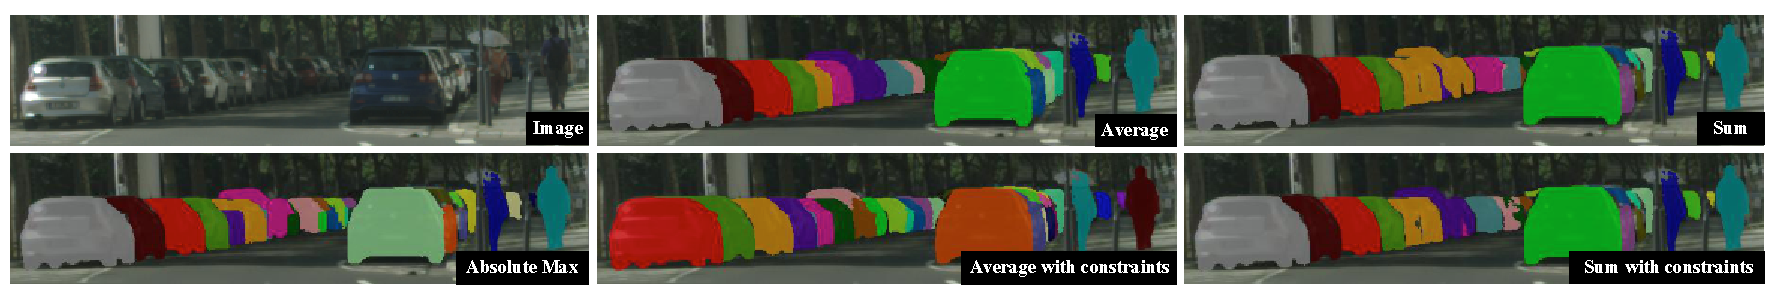
\includegraphics[width=\textwidth]{./figs/cityscapes_compare_4.pdf} % left bottom right top
\caption{Visual results given by different \algname{} linkage criteria on a crop of a CityScapes image}\label{fig:cityscapes}
\end{figure}
